\newpage
\section {Билет 5. Оптимизация запросов, построение и оценка планов запросов.}

Операции сущетсвуют 2-ух типов: 
\begin{itemize}
	\item DML - это аббревиатура от языка манипулирования данными. Он используется для извлечения, хранения, изменения, удаления, вставки и обновления данных в базе данных.
	
	Примеры: операторы SELECT, UPDATE, INSERT, DELETE, MERGE
	
	\item DDL - это аббревиатура языка определения данных. Он используется для создания и изменения структуры объектов базы данных в базе данных.
	
	Примеры: операторы CREATE, ALTER, DROP
\end{itemize}


SELECT - самый важный из DML

SELECT поля

FROM таблица 

WHERE условия 

Тут еще можно ипользовать GROUP BY и HAVING - поробно не обусждали 
\\[10pt]
1)\textbf{Способы соединение таблиц }

Хотим понять каким способом делать соединения таблиц. Пксть хотим соеденить 2 таблицы по id, те по A.id = B.id с условием A.a = x, B.b = y.

\textit{Способ 1}: \textbf{nested loop (вложенный цикл)}

Выбрать все данные из одной таблицы (например А по условию A.a= x) после этого для каждого id выбрать все подходящие из B (по индексу и значению B.b = y). По фатку это 2 цикла вложенных в друг друга..

Сложность: $N^2$ или на другой лекции $N_A * M_{id}$  -  кол записей отфильтрованных в таблице A * сложность доступа к таблице M по индексу. Если критерий x является очень хороший, то сложность становиться N. 

\textit{Способ 2}: \textbf{merge join (слияние)}

Взять наши данные и отфильтровать отдельно по условию x в таблице А, по условию y в таблице В, а дальше отсортировать и после этого соеденить два отсортированных массива.

Сложность: $NLogN$  или на другой лекции $NLogN * MLogM$. Если критерий x является очень хороший, а таблица В большая, то сложность останется такой же. 

Из-за этого нельзя сказать, какой способ (1 или 2) лучше. 

\textit{Способ 3}: \textbf{hash join (хеширование)}

При соединении хешированием строки одного набора помещаются в
хеш-таблицу, содержащуюся в памяти, а строки из второго набора
перебираются, и для каждой из них проверяется наличие
соответствующих строк в хеш-таблице.

Ключом хеш-таблицы является тот столбец, по которому выполняется
соединение наборов строк.

Такой способ эффективен для больших выборок. 
\\[15pt]
2) \textbf{Способы доступа к данным таблицы}

Теперь мы хотим выполнять запросы к одной таблице. У нас остается A.a= x. 

\textit{Способ 1}: \textbf{full scan} - проходить таблицу целиком. 

\textit{Способ 2}: \textbf{index} - используем индекс, если нужное значение заиндексировано и мы ищем какой-то диапозон. 

Пример: номер зачетки заиндексирован, и мы просто хотим найти номер зачетки, который равен x или находится в каком-то диапозоне. 

\textit{Способ 3}: \textbf{index scan} - предположим, что значение заиндексировано, а мы, например, хотим выбирать по значениям какой-то функции от значения в таблице, сам идекс такого не даст. Так что нам придется в любом случае читать данные. Вся запись весит много, а вот индекс, который хранит данные только одного значения, по факту весит гораздо меньше. 

Был пример с зачетками: заиндексирован номер зачетки, хотим получить человека с номером зачетки таким, что Sin от номера зачетки лежит в [0.5, 0.6], сам идекс такого не даст. Индекс хранить только номера зачеток, а полная запись содержит ФИО, место рождения, дату рождения и еще много всего. Соответсвенно, занимает много памяти и времени, если все читать из памяти для поиска, а в индесе мы читаем только номер зачетки, что весит гораздо меньше -> быстрее. 

\begin{figure}[H]
	\centering
	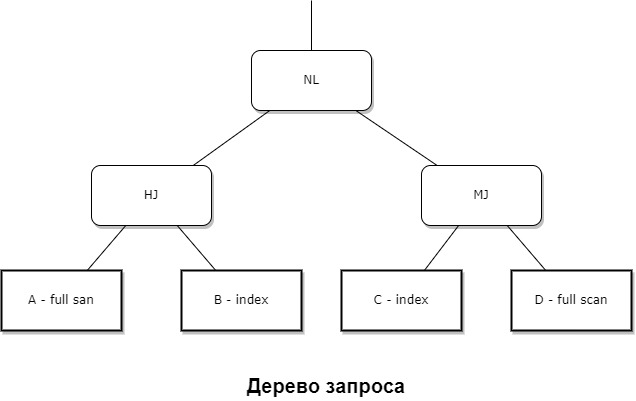
\includegraphics[scale = 0.5]{5/plan.jpg}
	\label{fig:plan1}
	\caption{}
\end{figure}

Пусть у нас есть запрос, в котором присутсвуют таблицы A, B, C, D. Нужно построит план выполнения запроса, которое выглядит как дерево. (Это не синтаксический разбор!). Тут мы решили отсканировать A full scan, B по индексу, а потом сделать между ними hash join. Рис. \ref{fig:plan1}

Скорость выполнения ОЧЕНЬ сильно зависит от оптимальности плана запроса.


Для выбора плана запроса в базе данных сущетсвует \textbf{оптимизатор}. Он получает на вход разобранный синтаксически SELECT и выдает план выполнения запроса (внутри оптимизатора еще правоверяются права доступа). 
\\[60pt]
\textbf{Виды оптимизаторов:} 
\textbf{Rule (cинтаксический)}. Основан на словарях, для того, чтобы выбрать лучший план запроса просмтатривает все условия, которые фигурируют в запросе и проводит анализ без учета данных (только на объялении структуры). Например в нем прошито правило, что индексный поиск по уникальному индексу - наилучший, после него идет не уникальный индекс, потом индекс скан, а потом фулл скан. Правил около 15, но суть одна (по факту прописаны приоритеты). Работает это очень быстро, но наилучший план он выбрать не может.

Почему плохой оптимизатор: мы хотим найти в базе студентов Ианова Рамиля, тогда нам выгодно в первую очередь искать по имени, так как Ивановых скорее всего много. Этот оптимизатор такое не учитывает. 

\textbf{Cost} Строит много планов выполнения запроса и считает их стоимость. По факту делает "виртуальное" выполнение запроса. У него есть оценки сколько понадобится сделать действий, чтобв прозвести какой-либо способ доступа. 

Нпример, если в оптимизаторе есть информация, что в таблице 1к блоков и в ней 1 миллион записей при этом уникальных 100к, тогда full scan должен прочитать все блоки и выбрать где-то 10 записей. Если же будет использоваться индекс, то нужно будет прочитать 10 блоков и выбрать 10 записей. 

Так для каждого плана появляется цена выполнения. Рассмотрим oracle: при расчете стоимости все операции (чтение диска, стоимость сортировки, процессорное время...) конвертируются в некоторую условную "валюту" , которая называется \textbf{логическим чтением блоков}. Стоимость высчитывается в этой валюте. Часто планы запроса хранятся, чтобы не пересчитываться много раз. 

Сложности: 

1) количество вариантов возможных планов запросов. Из-за этого оптмизатор работает классическими алгоритмами частичного обхода дерева (что-то вроде берутся наилучшие ветки, начинаем спуск, если оказалась сразу плохой, то мы ее откидываем и дальше не проверяем). И еще можно поставить ограничение на кол-во вариантов. 

2) Где брать данные, чтобы понимать, сколько мы получим записей после какой-то выборки. Если мы выбираем по фиксированным условиям (имя = Петр), то помогают строим гистограммы: по каждому столбцу строим общие характеристики и строим гистограммы сколько значений попадают в какой-то диапозон (на букву П у нас 8м записей, на букву К 10м и тд). Это частично решает проблему (так как строить уникальные гистограммы слишком затратно). 

Статистика не работает, если мы используем ограничения, которые невозможно заранее просчитать. Таких бывает 3 вида: 
\begin{enumerate}
	\item Для столбцов, которые имеют близкие значения с очень разнми частотами.
	\item использование ограничений, которые содержат функцию (хотим выбрать студентов у которых третий знак после запятой в синусе от веса студента равен 3, понятно, что гистограмма бесполезна) 
	\item (самый важный для нас) Если мы имеем дело с доступом к удаленным данным: получаем данные с другого сервера, но статистики его мы не знаем.
\end{enumerate}

Есть два подхода к решению таких сложностей: 

\begin{enumerate}
	\item Семплирование - получение примера данных. (Например в oracle: A SAMPLE (5) - хотим счиать из таблицы 5\% случайных блоков). Берутся примеры данных из всех таблиц, и на них проверяются условия выборки. Потом расширяем полученные данные на всю таблицу и считаем, что получили всю статистику. (для удаленных данных просто просим прислать какой-то поцент блоков и далее аналогично). Способ хороший так как дает +- точные результаты, но есть недостаток - стоимость подготовки плана (может присылаться очень много данных).
	\item Перестаивание дерева находу. Реализуется сложно, но принцип простой:  смотрим на картинку плана запроса. Мы предполагаем, что при объединении (HJ) А и В мы получим примерно 4 записи (не стоимость) и тогда выше стоящий NL оптимальный вариант. Начали выполнять, в момент соединения А и В HJ мы получили 400к записей и в таком случае система останавливает выполнение запроса и производит пересчет кусков, которые мы еще не выполнили.
\end{enumerate}

Существует еще один метод оптимизации запроса - \textbf{переписывание}. 

Вспоминаем три структуры данных: \textit{таблицы} - просто хранят данные, \textit{представления} - запросы к таблицам (возможно, в виде плана запроса), \textit{материальные представления} - результат выполнения какого-то запроса. 

Нас интересуют материальные представения. У мп есть метка вычисления (мы можем сказать, когда менялись таблицы и когда было посчитано материальное представление). Смотрим на рисунок плана. Пусть мы захотели отдельно посмотреть HJ для A и В. Если HJ был сделан после изменения таблиц, то мы можем удалить часть дерева ниже HJ и подставить туда материальное представление ( Рис.\ref{fig:plan2}). Так мы сокращаем размер вычислений.  

\begin{figure}[H]
	\centering
	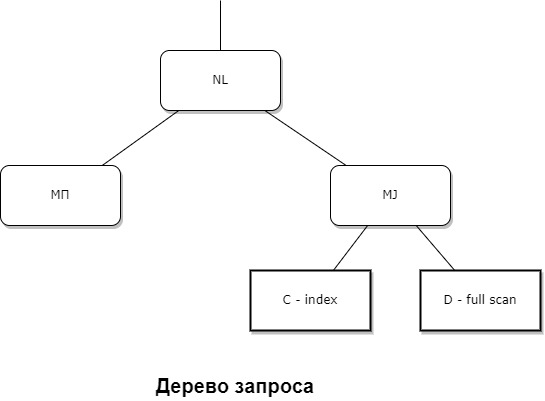
\includegraphics[scale = 0.5]{5/plan2.jpg}
	\label{fig:plan2}
	\caption{после добавления МП}
\end{figure}

\color{blue} Дальше говорим про удаленное выполнение запроса, не знаю, надо ли, но в билете нет. Если интересно 3 семинар, 29 минута. Тут напишу краткий список. 
\color{black}

Механизмы получения данных из внешней системы (териналогия  oracle)
\begin{itemize}
	\item  dblink -  связывают бд одного типа (умеюст все делать так как все друг о друге знают)
	\item внешние таблицы - если надо подключить статические данные (например csv файл). Может быть медленным, особо ничего нет
	\item шлюзы (ODBC) 
\end{itemize}